\documentclass[onecolumn, draftclsnofoot,10pt, compsoc]{IEEEtran}
\usepackage{graphicx}
\usepackage[section]{placeins}
\usepackage{url}
\usepackage{setspace}
 
\usepackage{alltt}                                           
\usepackage{float}
\usepackage{color}
\usepackage{url}

\usepackage{geometry}
\geometry{textheight=9.5in, textwidth=7in}
\setlength\parindent{0pt}

\usepackage{xspace}
\usepackage{pgfgantt}
\usepackage{subcaption}

% 1. Fill in these details
\def \CapstoneTeamName{\textbf{Insert Team Name Here} }
\def \CapstoneTeamNumber{8}
\def \GroupMemberOne{James Stallkamp}
\def \GroupMemberTwo{Jeremy Fischer}
\def \GroupMemberThree{Austin Row}
\def \CapstoneProjectName{NLP For Digital Manufacturing}
\def \CapstoneSponsorCompany{Autodesk}
\def \CapstoneSponsorPerson{Patti Vrobel}
\def \botname{Kora\xspace}

% 2. Uncomment the appropriate line below so that the document type works
\def \DocType{		%Problem Statement
				Requirements Document
				%Technology Review
				%Design Document
				%Progress Report
				}
			
\newcommand{\NameSigPair}[1]{\par
\makebox[2.75in][r]{#1} \hfil 	\makebox[3.25in]{\makebox[2.25in]{\hrulefill} \hfill		\makebox[.75in]{\hrulefill}}
\par\vspace{-12pt} \textit{\tiny\noindent
\makebox[2.75in]{} \hfil		\makebox[3.25in]{\makebox[2.25in][r]{Signature} \hfill	\makebox[.75in][r]{Date}}}}
% 3. If the document is not to be signed, uncomment the RENEWcommand below
\renewcommand{\NameSigPair}[1]{#1}

%%%%%%%%%%%%%%%%%%%%%%%%%%%%%%%%%%%%%%%
\begin{document}
\begin{titlepage}
    \pagenumbering{gobble}
    \begin{singlespace}
    	
\includegraphics[height=4cm]{coe_v_spot1}
        %\hfill 
        % 4. If you have a logo, use this includegraphics command to put it on the coversheet.
        
\includegraphics[height=4cm]{autodesk}   
        \par\vspace{.2in}
        \centering
        \scshape{
            \huge CS Capstone \DocType \par
            {\large\today}\par
            \vspace{.5in}
            \textbf{\Huge\CapstoneProjectName}\par
            \vfill
            {\large Prepared for}\par
            \Huge \CapstoneSponsorCompany\par
            \vspace{5pt}
            {\Large\NameSigPair{\CapstoneSponsorPerson}\par}
            {\large Prepared by }\par
            Group\CapstoneTeamNumber\par
            % 5. comment out the line below this one if you do not wish to name your team
            %\CapstoneTeamName\par 
            \vspace{5pt}
            {\Large
                \NameSigPair{\GroupMemberOne}\par
                \NameSigPair{\GroupMemberTwo}\par
                \NameSigPair{\GroupMemberThree}\par
            }
            \vspace{20pt}
        }
        \begin{abstract}
       		This document outlines the technical requirements that \botname must meet before the 2018 OSU Engineering Expo. 
            It starts with an overall description of the project and follows with specific functional and performance requirements.
            At the end, there is a Gantt chart which gives a timeline detailing when each major requirement will be completed.
        \end{abstract}     
    \end{singlespace}
\end{titlepage}
\newpage
\pagenumbering{arabic}
\tableofcontents
% 7. uncomment this (if applicable). Consider adding a page break.
%\listoffigures
%\listoftables
\clearpage

% 8. now you write!
\section{Introduction}
        The introduction outlines the purpose and scope of the project. 
        This section is also responsible for defining any prerequisite acronyms and terms used in the document. 
    \subsection{Purpose}
        The purpose of this document is to specify the exact requirements that \botname must meet to be considered a successful project. 
        This document is a mutual agreement between the client and developers regarding the expected result of this project.
        The intended audience is the two aforementioned parties.
    \subsection{Scope}
        \botname will be a speech-based virtual assistant for Fusion that lets users perform any one of a subset of tasks within the product, such as saving a document or opening a menu, by verbally instructing it to perform the task.
        Workflows in Fusion that are not suited for handling by a voice interface will not be supported by \botname.
        As a stretch goal, \botname will be capable of questioning the user and using responses to predict and automatically assist with future user behavior.
        It will be a plugin that is bundled with Fusion and will be part of the product's standard download. \\

        \botname will offer users a tool that decreases the time required to achieve their goals within Fusion by offering an interface that runs in parallel with and complements the keyboard and mouse.
        If the stretch goal is achieved, \botname will further increase productivity by learning to predict and automate specific workflows within the product.
        

    \subsection{Definitions, Acronyms, and Abbreviations}
        \begin{table}[h]
            \centering
            \caption{Definitions}
            \label{my-label}
            \begin{tabular}{|l|l|}
                \hline
                \textbf{Term} & \textbf{Definition} \\ \hline
                \botname & The virtual assistant that is the focus of this project \\ \hline
                NLP & Natural Language Processing \\ \hline
                API & Application Programing Interface \\ \hline
                CAD & Computer Aided Design \\ \hline
                CAM & Computer Aided Manufacturing \\ \hline
                Fusion & An Autodesk Cloud-based 3D CAD/CAM tool/product \\ \hline
                Task & In the context of Fusion, a function or operation that can be performed in Fusion \\ \hline
                Plugin & Software that adds specific new functionlity to another piece of software \\ \hline
                User & A person that interacts with \botname or Fusion depending on the context \\ \hline
                Workflow & A sequence of related tasks \\ \hline
            \end{tabular}
        \end{table}
    %\subsection{References}
        %TODO
    \subsection{Overview}
        %This section describes the contents and organization of the rest of the document. 
        The rest of this document outlines intended uses and specific functionalities of \botname as well as assumptions, dependencies, and constraints that pertain to the project. 

\section{Overall Description}
    \subsection{Product Perspective}

        %\subsubsection{System Interfaces}
            %TODO: Revisit this. I'm not sure if it is applicable to this project.
        \subsubsection{User Interfaces}
            The user will interact with \botname via voice commands given in English. 
            To initiate a command, the user will say "\botname" followed by the command. \\

            As part of a stretch goal, \botname will periodically ask questions back to the user via a speech synthesizer.

        \subsubsection{Hardware Interfaces} 
            \botname will be supported on desktop and laptop computers that support Fusion and have microphones to receive the user's speech.
            For stretch goal support, devices will also need speakers through which \botname can speak back to the user.

        \subsubsection{Software Interfaces}               
            \botname needs to translate supported speech commands received from the user to the equivalent tasks within the user's Fusion project.
            For this, a series of open source NLP projects will be linked to derive meaning from speech.
            The derived meaning will then be mapped to a Fusion API call.
        %\subsubsection{Communications Interfaces}                

        %\subsubsection{Operations}
            %TODO: I'm not sure what this section means.

        \subsubsection{Site Adaptation Requirements} 
            Since \botname interacts with Fusion using existing architecture, Fusion will not need to be modified to support it. 

    \subsection{Product Functions}
        \botname will allow the user to perform tasks in Fusion via a voice interface. 
        Each voice command given by the user will be mapped to a specific task which will then be performed in the open Fusion project. \\
       
        As a stretch goal, \botname will periodically ask the user questions regarding why they have performed specific tasks.
        The questions asked by \botname will pertain to specific predefined contexts.
		\botname will record user responses and save a transcript along with contextual information.
        Responses will also be used to try to predict and assist with future user actions. \\

        All interactions with \botname will be logged for debugging and future development purposes.
        
    \subsection{User Characteristics}
		\botname will have two types of users: administrators and designers. 
		Administrators will have access to data collected by \botname including the command logs and, if the stretch goal is accomplished, user responses to questions from \botname. \\
		
		The primary user is the designer who is working on projects inside of Fusion. 
        Due to the technical knowledge needed to work within Fusion, it can be assumed that designers are technically oriented.
        However, no extra knowledge outside of that needed to operate Fusion will be needed to operate \botname.
        
    \subsection{Constraints}
        \botname will not be integrated with the Fusion source code and thus will be constrained in what tasks it can perform by what is offered in the Fusion API. 

    \subsection{Assumptions and Dependencies}
        Since this project does not focus on developing software to handle speech recognition and natural language processing, it depends on the existence of adequate open source resources for handling this aspect of \botname. \\

        The stretch goal assumes that the Fusion API offers a way to view actions that the user performs with their keyboard and mouse.
        Without this capability, the application's knowledge of user actions will be limited to the actions that the user performs through \botname.

\section{Specific Requirements}
    \subsection{External Interface}
       After \botname is released, Fusion users will be shown a modal the next time that they log into the product that gives a brief description of \botname and asks if they would like to enable it.
       If a user chooses not to enable \botname, their Fusion editor environment will not be changed. \\

       Users that enable \botname will be presented with an onboarding process that incorporates an interactive demo.
       The onboarding process will start with a popup that introduces \botname with a concise description of its purpose.
       The user will then be able to click "Next" to transition to an interactive demo.
       The interactive demo will consist of several sequential popups that each ask the user to tell \botname to perform a specific command.
       This will make the user aware of \botname and the functionality that it offers.

    \subsection{Functional Requirements}
    This section includes the requirements that specify all the fundamental actions of the software system.
        \subsubsection{Functional Requirement 1}
        TITLE: Status Messaging \\
        DESCRIPTION: The system shall alert the user when it has understood a command as well as when it has failed to interpret a user command or has reached an error state. \\
        RATIONALE: This clarifies for the user if \botname is doing what they think it should be doing or if they need to try again. 
        
        \subsubsection{Functional Requirement 2}
        TITLE: Extrude \\
        DESCRIPTION: \botname shall be able to extrude a selected face. \\
        RATIONALE: This is a task that users perform often.
        
        \subsubsection{Functional Requirement 3}
        TITLE: Rotate Camera \\
        DESCRIPTION: \botname shall be able to rotate the Fusion camera. \\
        RATIONALE: This is a task that users perform often.
        
        \subsubsection{Functional Requirement 4}
        TITLE: Save Project \\
        DESCRIPTION: \botname shall be able to save a Fusion project. \\
        RATIONALE: This is a task that users perform often.
        
        \subsubsection{Functional Requirement 5}
        TITLE: Logging User Interactions \\
        DESCRIPTION: \botname shall log every interaction that a user has with it and the result of that interaction. \\
        RATIONALE: This offers helpful information for debugging purposes. This information can also be used to learn how \botname is being used and to drive future development.
       
        \subsubsection{Functional Requirement 6}
        TITLE: Command Signalling \\
        DESCRIPTION: \botname will begin listening for a command after hearing the user say "\botname". \\
        RATIONALE: This is a pattern that is used in many successful voice assistants to signal when to start listening for a command.

        %	%
        %	Below are stretch goals
        %	%
        
        \subsubsection{Stretch Functional Requirement 1}
        TITLE: Smart Assistant \\
        DESCRIPTION: \botname will be able to offer executable suggestions in the form of "Would you like to...?" questions that the user will respond in the affirmative to at least 15\% of the time. \\
        RATIONALE: This is the ultimate vision for \botname in which it can predict what the user will want to do next and will be able to perform those next steps for the user. 
        
    \subsection{Performance Requirements}
        The section lists the performance requirements that will be met by \botname.
        
        \subsubsection{Performance Requirement 1}
        TITLE: Response Time \\
        DESCRIPTION: It will take a user at most one second longer to perform a supported task through \botname than it would take when using a keyboard and mouse. \\
        RATIONALE: The user must feel that \botname enhances rather than slows their development speed.
        
    \subsection{Design Constraints}
        \botname will execute tasks in Fusion via the Fusion API. 
        Therefore supported tasks will constrained to those capable of being performed by the API.
        
\section{Release Plan}

    \subsection{Release plan}
    	\begin{figure}[H]
            \begin{center}
                %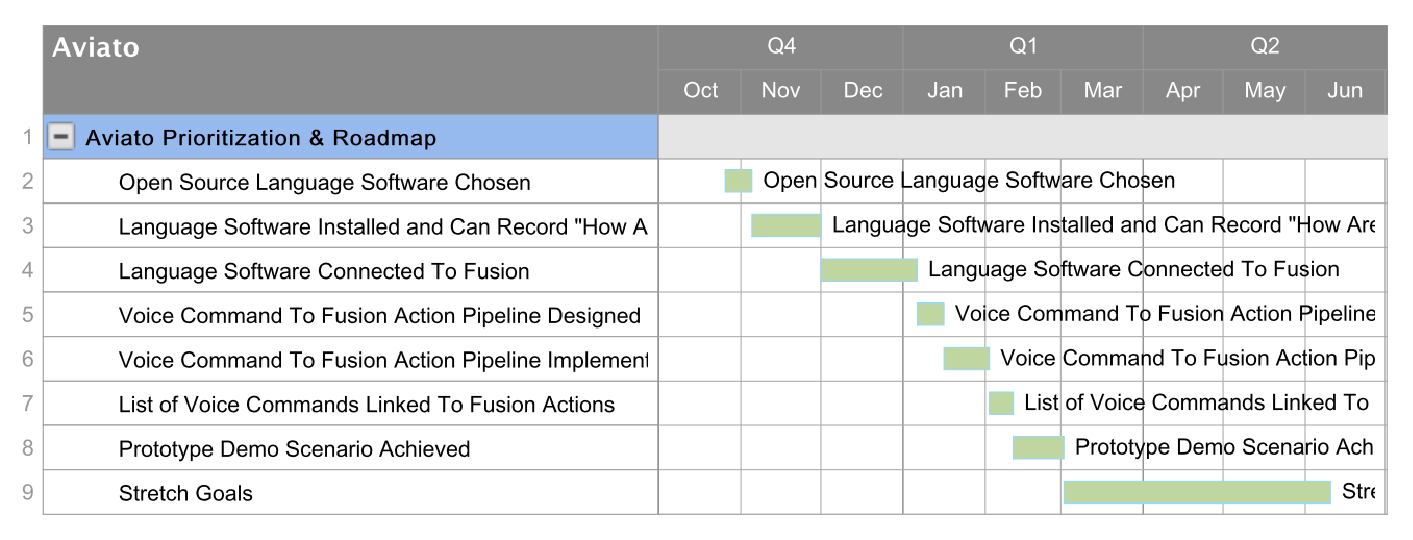
\includegraphics[width=1\textwidth]{ganttChart.eps}
                %Changed Gantt chart to be modifiable.
                \begin{ganttchart}[
                        y unit title=0.4cm,
                        y unit chart=0.5cm,
                        vgrid,
                        hgrid,
                        title left shift=.05, 
                        title right shift=.05, 
                        title height=1, 
                        group right shift=0
                    ]{1}{28}
                    \gantttitle{Months}{28} \\
                    \gantttitle{October}{4}
                    \gantttitle{November}{4}
                    \gantttitle{December}{4}
                    \gantttitle{January}{4}
                    \gantttitle{February}{4}
                    \gantttitle{March}{4}
                    \gantttitle{April}{4} \\

                    \ganttbar{Problem Statement}{1}{2} \\
                    \ganttbar{Requirements Document}{3}{4} \\
                    \ganttbar{Technology Review}{5}{6} \\
                    \ganttbar{Design \botname}{7}{8} \\
                    \ganttbar{Fall Progress Report}{9}{9} \\
                    \ganttbar{Speech-to-Task Pipeline}{10}{14} \\
                    \ganttbar{Create Alpha Demo}{18}{18} \\
                    \ganttbar{Train NLP Modules}{13}{25} \\
                    \ganttbar{Performance Testing}{16}{25} \\
                    \ganttbar{Create Beta Demo}{22}{22} \\
                    \ganttbar{Smart Assistant Stretch Goal}{15}{23} \\
                    \ganttbar{Engineering Expo}{26}{26} \\

                \end{ganttchart}
                \captionsetup{justification=centering}
                \caption{\botname Development Schedule}
                \label{fig:developmentSchedule1}
            \end{center}
    	\end{figure}


%\bibliography{requirementsBib} 
%\bibliographystyle{ieeetr}

\end{document}
